\documentclass[../../main.tex]{subfiles}

\begin{document}
    \section{False Sharing, Race Conditions, and Schedules}
    \subsection{False Sharing}
    Consider two teachers who need to count their students. To divide the work, one teacher decides to count the boys, while the other counts the girls. They use a single sheet of paper to keep track, marking a stroke on their respective sides of the page for each student they count.
    
    ~\\
    However, even though they each have their own pen, they're still working with only one piece of paper. This setup means that every time one teacher wants to make a mark, they must pass the paper to the other, as both are using different parts of the same sheet.

    ~\\
    This constant handoff slows them down significantly. Had they used separate sheets, they could each count freely without interrupting one another.

    ~\\
    In the same way, false sharing occurs in computing when multiple threads modify different parts of the same cache line. Even though each thread may be working on separate variables, they're forced to constantly invalidate and reload the cache line they "share", leading to substantial inefficiencies.

    ~\\
    Here is an illustration of the scenario:

    \begin{figure}[h]
        \centering
        \resizebox{\textwidth}{!}{
            \begin{tikzpicture}
                % Paper
                \draw[thick] (0, 0) rectangle (6, 3);
                \node[above] at (3, 3) {Shared Paper};

                % Divider line
                \draw[dashed] (3, 0) -- (3, 3);
                
                % Labels for boys' and girls' side
                \node at (1.5, 1.5) {Boys' Count Side};
                \node at (4.5, 1.5) {Girls' Count Side};

                % Teacher 1
                \node[draw, rectangle, minimum width=2cm, minimum height=1cm, fill=blue!20] (teacher1) at (-3, 1.5) {Teacher 1};
                \node[below=0.1cm of teacher1] {Counting Boys};
                \draw[->, thick] (teacher1.east) -- (-0.2, 1.5);

                % Teacher 2
                \node[draw, rectangle, minimum width=2cm, minimum height=1cm, fill=red!20] (teacher2) at (9, 1.5) {Teacher 2};
                \node[below=0.1cm of teacher2] {Counting Girls};
                \draw[->, thick] (teacher2.west) -- (6.2, 1.5);
                
                % Arrows to represent passing the paper
                % \draw[<->, thick, dashed] (teacher1.east) -- node[above]{Pass Paper} (teacher2.west);
            \end{tikzpicture}
        }
        \caption{False Sharing Analogy: Two teachers repeatedly passing a single paper to count students separately.}
    \end{figure}

    \newpage
    \subsection{There's plenty of room at the Top}
    Let us analyze the following graphic from the paper \em There’s plenty of room at the Top: What
will drive computer performance after Moore’s law? \em:

    ~\\
    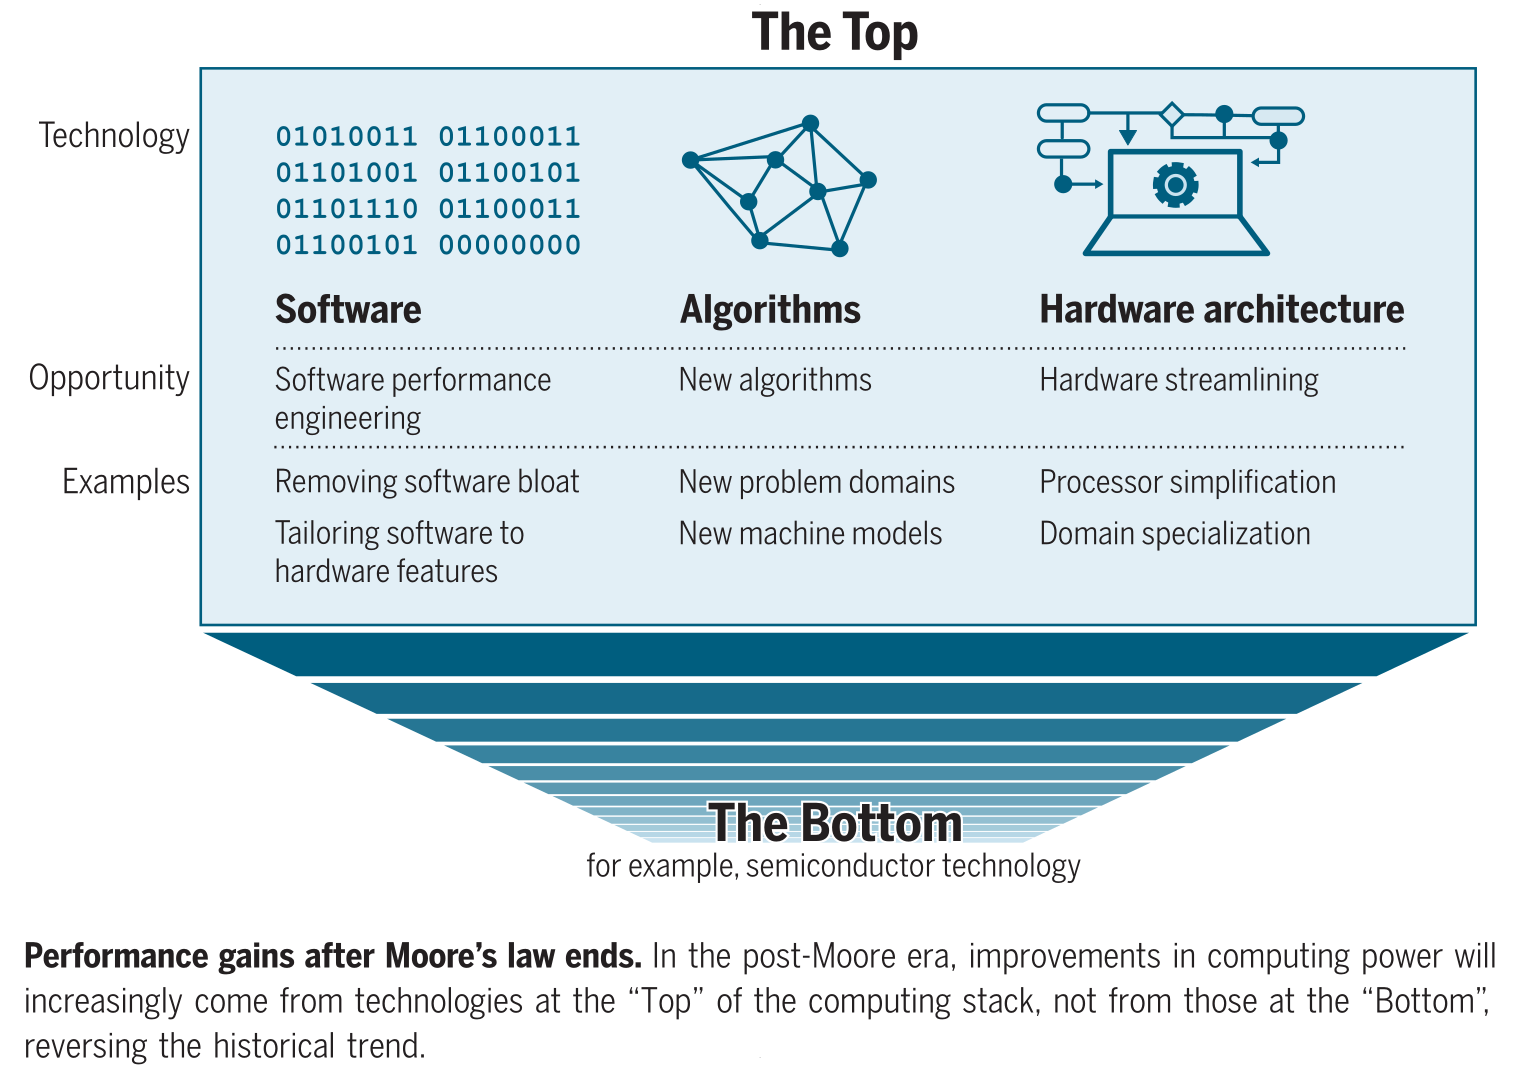
\includegraphics[width=\textwidth]{chapters/02/more_room_at_the_top.png}

    ~\\
    The entire blue area basically represents the foundation of running software:
    We need hardware ("The Bottom") as well as good software ("The Top").
    The width represents the potential of gains we could make in these areas.
    In particular, the width of "The Bottom" shrank over time and is now becoming less significant.

    ~\\
    The paper assumes that the most potential lies in the three categories \em Software, Algorithms, and Hardware Architecture\em, all of which are located at The Top.
    They describe their potentials in the \em Opportunity \em and \em Examples \em fields. Let us analyze them individually:

    ~\\
    \subsubsection{Software}
    The software that is ultimately run on the hardware can be optimized itself.
    In Software Engineering, there is a phenomenon called \emph{bloat}.
    It describes the accumulation of unnecessary functionality and features, which makes programs bigger and hence slower.
    By carefully writing code to avoid these traps, we can improve the running time of our programs.

    ~\\
    Tailoring software to hardware features allows developers to leverage specific capabilities of the underlying hardware. For instance, optimizing software to use SIMD (Single Instruction, Multiple Data) instructions can dramatically increase performance for tasks that involve large data sets, such as graphics processing or numerical simulations. Additionally, understanding cache architectures can help developers design algorithms that reduce cache misses, leading to faster data access and processing. By aligning software architecture with hardware capabilities, significant improvements in execution speed and resource utilization can be achieved.

    ~\\
    \subsubsection{Algorithms}
    The choice of algorithms plays a critical role in determining software performance. Implementing new algorithms that are more efficient in terms of time and space complexity can lead to significant performance enhancements. For example, employing faster sorting algorithms or utilizing data structures that provide quicker access times can reduce the computational overhead. 

    ~\\
    New problem domains often introduce unique challenges that require innovative algorithmic solutions. For instance, the advent of big data has prompted the development of algorithms specifically designed for distributed computing environments, which can process large datasets across multiple machines. By addressing the specific needs of these new domains, developers can create algorithms that are optimized for performance and scalability.

    ~\\
    \subsubsection{Hardware Architecture}
    Hardware streamlining involves optimizing hardware components to enhance overall system performance. This can include reducing the complexity of circuits, minimizing power consumption, and improving thermal management. Streamlined hardware can lead to faster processing speeds and better energy efficiency, directly impacting software performance by reducing bottlenecks.

    ~\\
    Processor simplification is another approach to improving performance. By reducing the number of transistors or focusing on a reduced instruction set, processors can operate at higher speeds and with lower power consumption. Simplified processors are often easier to design, implement, and manufacture, which can also reduce costs while enhancing performance metrics.

    ~\\
    Domain specialization allows hardware to be optimized for specific applications or problem domains. For example, graphics processing units (GPUs) are designed to handle complex graphics calculations more efficiently than general-purpose CPUs. Similarly, application-specific integrated circuits (ASICs) can be tailored for particular tasks, such as cryptocurrency mining or machine learning inference, resulting in substantial performance gains over generic hardware solutions.

    \newpage
    \subsection{Parallelizing pi\_numerical\_integration.cpp}
    Here is the parallelized version using the \em \#pragma omp for \em construct:

    \smallbreak
    \smallbreak
    \begin{samepage}
    \begin{lstlisting}
#include <iomanip>
#include <iostream>
#include <omp.h>

using namespace std;

int main() {
    int num_steps = 100000000; // number of rectangles
    double width = 1.0 / double(num_steps); // width of a rectangle
    double sum = 0.0; // for summing up all heights of rectangles

    double start_time = omp_get_wtime(); // wall clock time in seconds
    #pragma omp parallel for reduction(+:sum)
    for (int i = 0; i < num_steps; i++) {
        double x = (i + 0.5) * width; // midpoint
        sum = sum + (1.0 / (1.0 + x * x)); // add new height of a rectangle
    }
    double pi = sum * 4 * width; // compute pi
    double run_time = omp_get_wtime() - start_time;

    cout << "pi with " << num_steps << " steps is " << setprecision(17)
        << pi << " in " << setprecision(6) << run_time << " seconds\n";
}
    \end{lstlisting}
    \end{samepage}
\end{document}